%%%%%%%%%%%%%%%%%%%%%%%%%
% Dokumentinformationen %
%%%%%%%%%%%%%%%%%%%%%%%%%
\newcommand{\titleinfo}{Nachrichtentechnik 1 - Formelsammlung}
\newcommand{\authorinfo}{Braun \& Co, J.Rast}
\newcommand{\versioninfo}{$Revision: 1 $ - powered by \LaTeX}

%%%%%%%%%%%%%%%%%%%%%%%%%%%%%%%%%%%%%%%%%%%%%
% Standard projektübergreifender Header für
% - Makros 
% - Farben
% - Mathematische Operatoren 
%
% DORT NUR ERGÄNZEN, NICHTS LÖSCHEN
%%%%%%%%%%%%%%%%%%%%%%%%%%%%%%%%%%%%%%%%%%%%%  
% Genereller Header
\documentclass[10pt,twoside,a4paper,fleqn]{article}
% Dateiencoding
\usepackage[utf8]{inputenc}
% Seitenränder
\usepackage[left=1cm,right=1cm,top=1cm,bottom=1cm,includeheadfoot]{geometry}
% Sprachpaket
\usepackage[ngerman]{babel,varioref}

% Pakete
\usepackage{amssymb,amsmath,fancybox,graphicx,lastpage,wrapfig,fancyhdr,hyperref,verbatim,floatflt,multicol,multirow,rotating,pdflscape,array,longtable,listings, enumitem, textcomp}

% Zum Bilder einfach in Tabellen einfügen (valign=t)
\usepackage[export]{adjustbox}

%%%%%%%%%%%%%%%%%%%%
% Generelle Makros %
%%%%%%%%%%%%%%%%%%%%
\newcommand{\skript}[1]{$_{\textcolor{red}{\mbox{\small{Skript S.#1}}}}$}
\newcommand{\verweis}[2]{\small{(siehe auch \ref{#1}, #2 (S. \pageref{#1}))}}
\newcommand{\verweiskurz}[1]{(\small{siehe \ref{#1}\normalsize)}}
\newcommand{\subsubadd}[1]{\textcolor{black}{\mbox{#1}}}
\newcommand{\formelbuch}[1]{$_{\textcolor{red}{\mbox{\small{S#1}}}}$}

\newcommand{\kuchling}[1]{$_{\textcolor{red}{\mbox{\small{Kuchling #1}}}}$}
\newcommand{\stoecker}[1]{$_{\textcolor{orange}{\mbox{\small{Stöcker #1}}}}$}
\newcommand{\sachs}[1]{$_{\textcolor{blue}{\mbox{\small{Sachs S. #1}}}}$}
\newcommand{\hartl}[1]{$_{\textcolor{green}{\mbox{\small{Hartl S. #1}}}}$}

\newcommand{\schaum}[1]{\tiny Schaum S. #1}

\newcommand{\skriptsection}[2]{\section{#1 {\tiny Skript S. #2}}}
\newcommand{\skriptsubsection}[2]{\subsection{#1 {\tiny Skript S. #2}}}
\newcommand{\skriptsubsubsection}[2]{\subsubsection{#1 {\tiny Skript S. #2}}}

\newcommand{\matlab}[1]{\footnotesize{(Matlab: \texttt{#1})}\normalsize{}}

%%%%%%%%%%
% Farben %
%%%%%%%%%%
\usepackage{xcolor}

%%%%%%%%%%%%%%%%%%%%%%%%%%%%
% Mathematische Operatoren %
%%%%%%%%%%%%%%%%%%%%%%%%%%%%
\DeclareMathOperator{\sinc}{sinc}
\DeclareMathOperator{\sgn}{sgn}
\DeclareMathOperator{\Real}{Re}
\DeclareMathOperator{\Imag}{Im}
%\DeclareMathOperator{\e}{e}
\DeclareMathOperator{\cov}{cov}
\DeclareMathOperator{\PolyGrad}{PolyGrad}

%Makro für 'd' von Integral- und Differentialgleichungen 
\newcommand*{\diff}{\mathop{}\!\mathrm{d}}


%%%%%%%%%%%%%%%%%%%%%%%%%%%
% Fouriertransformationen %
%%%%%%%%%%%%%%%%%%%%%%%%%%%
\usepackage{trfsigns, trsym}
%\unitlength1cm
% Zeitbereich -- Frequenzbereich
%\newcommand{\laplace}
%{
%\begin{picture}(1,0.5)
%\put(0.2,0.1){\circle{0.14}}\put(0.27,0.1){\line(1,0){0.5}}\put(0.77,0.1){\circle*{0.14}}
%\end{picture}
%}
% Frequenzbereich -- Zeitbereich
%\newcommand{\Laplace}
%{
%\begin{picture}(1,0.5)
%\put(0.2,0.1){\circle*{0.14}}\put(0.27,0.1){\line(1,0){0.45}}\put(0.77,0.1){\circle{0.14}}
%\end{picture}
%}


% Fouriertransformationen
\unitlength1cm
\newcommand{\FT}
{
\begin{picture}(1,0.5)
\put(0.2,0.1){\circle{0.14}}\put(0.27,0.1){\line(1,0){0.5}}\put(0.77,0.1){\circle*{0.14}}
\end{picture}
}


\newcommand{\IFT}
{
\begin{picture}(1,0.5)
\put(0.2,0.1){\circle*{0.14}}\put(0.27,0.1){\line(1,0){0.45}}\put(0.77,0.1){\circle{0.14}}
\end{picture}
}




%%%%%%%%%%%%%%%%%%%%%%%%%%%%
% Allgemeine Einstellungen %
%%%%%%%%%%%%%%%%%%%%%%%%%%%%
%PDF Info
\hypersetup{pdfauthor={\authorinfo},pdftitle={\titleinfo},colorlinks=false}
\author{\authorinfo}
\title{\titleinfo}

%%%%%%%%%%%%%%%%%%%%%%%
% Kopf- und Fusszeile %
%%%%%%%%%%%%%%%%%%%%%%%
\pagestyle{fancy}
\fancyhf{}
%Linien oben und unten
\renewcommand{\headrulewidth}{0.5pt} 
\renewcommand{\footrulewidth}{0.5pt}

\fancyhead[L]{\titleinfo{ }\tiny{(\versioninfo)}}
%Kopfzeile rechts bzw. aussen
\fancyhead[R]{Seite \thepage { }von \pageref{LastPage}}
%Fusszeile links bzw. innen
\fancyfoot[L]{\footnotesize{\authorinfo}}
%Fusszeile rechts bzw. ausen
\fancyfoot[R]{\footnotesize{\today}}
% Lizenz CC-BY-NC-SA
% Headerfile für die Einbindung einer Lizenzgrafik in den Footer
% Verwendung: \lizenz{cc-by-nc-sa}{small}
\newcommand{\lizenz}[2]
{
\fancyfoot[C]{
  \includegraphics[width=1.6cm]{./header/lizenzen/#1/#2.png}
}
}
\lizenz{cc-by-nc-sa}{small}
% Einrücken verhindern versuchen
\setlength{\parindent}{0pt}

% Zeilenhöhe Tabellen:
\newcommand{\arraystretchOriginal}{1.5}
\renewcommand{\arraystretch}{\arraystretchOriginal}



% Möglichst keine Ergänzungen hier, sondern in header.tex
\begin{document} 
 

%%%%%%%%%%%%%%%%%%%%%%%%%%%%%%%%%%%%%%%%%%%%%%%%%%%%%%%%%%%%%%%%%%%%%%%%%%%%%%%%%%%%%%%%%%%%%%%
%%%%%%%%%%%%%%%%%%%%%%%%%%%%%%%%%%%%%%%%%%%%%%%%%%%%%%%%%%%%%%%%%%%%%%%%%%%%%%%%%%%%%%%%%%%%%%%
\section{Grundbegriffe}
\subsection{Einfaches Kommunikationsmodell}
\begin{center}
	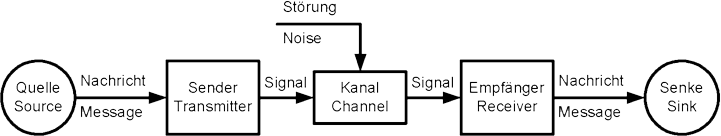
\includegraphics[width=14cm]{../NaT1/bilder/kommunikationsmodell.png}
\end{center}



\subsection{Pegel (Dezibel)}
\textbf{Mit Dezibel (dB) vergleicht man Leistungspegel, nicht Amplituden!}

\subsubsection{Relative Pegel}
	\begin{tabbing}
	xxxxxxxxxxxxxxxxxxxxxxxxx \= xxxxxxxxxxxxxxxxxxxxxxx  \= xxxxxxxxxxxxxxxxxxxxxxx \=\kill
	\textbf{Spannungspegel} \> $L_U = 20 \cdot \log_{10} \frac{U_x}{U_0}$ \> $U_x = U_0 \cdot
	10^{\frac{L_U}{20}} $ \> $[L_U] = dB$ \\ 
	\textbf{Strompegel} \> $L_I  = 20 \cdot \log_{10} \frac{I_x}{I_0}$ \> $I_x = I_0 \cdot
	10^{\frac{L_I}{20}} $ \> $[L_I] = dB$ \\ 
	\textbf{Leistungspegel} \> $L_P = 10 \cdot \log_{10} \frac{P_x}{P_0}$ \> $P_x = P_0 \cdot
	10^{\frac{L_U}{10}} $ \> $[L_P] = dB$
	\end{tabbing}

\subsubsection{Absolute Pegel}
	\begin{tabbing}
	xxxxxxxxxxxxxxxxxxxxxxxxx \= xxxxxxxxxxxxxxxxxxxxxxxxxxxxxxxxxxxxx  \= xxxxxxxxxxxxxxxxxxxxxxx \=\kill
	\textbf{dBW} \> Leistungspegel mit Bezugsgrösse $P_0 = $1W \> $\Longrightarrow \: 0 \: dBW = 1W$\\
	\textbf{dBm} \> Leistungspegel mit Bezugsgrösse $P_0 = $1mW \> $\Longrightarrow \: 0 \: dBm = 1mW$\\
	\textbf{dBV} \> Spannungspegel mit Bezugsgrösse $U_0 = $1V \> $\Longrightarrow \: 0 \: dBV = (1V)^2/R_{ref}$\\
	\textbf{dB}$\mu$V \> Spannungspegel mit Bezugsgrösse $U_0 = $1$\mu$V \> $\Longrightarrow \: 0 \: dB \mu V = (1 \mu V)^2/R_{ref}$
	\end{tabbing}
Bei \textbf{Spannungspegeln} (dBV, dB$\mu$V) muss immer der \textbf{Referenz-Widerstand} ($R_{ref}$) berücksichtigt werden: \\
In der \textbf{HF-Technik} üblich, $R_{ref} = 50 \Omega \Rightarrow 0 dBV = 20 mW \qquad $
In der \textbf{Telefonie} üblich, $R_{ref} = 600  \Omega \Rightarrow 0 dBV =
1.67 mW$ 

\subsection{Signalklassifizierungen}
Absoluter Werte des Signals sind irrelevant - Physikalische Dimension wird weggelassen. \\
Signal $x(t)$ wird auf $|x(t)| \leq 1$ normiert.

\renewcommand{\arraystretch}{2}
\begin{tabular}[c]{ | p{9cm} | p{9cm} | }
\hline
	\begin{minipage}[t]{9cm}
		\textbf{Leistung} \\
		$ P = \lim \limits_{T \to \infty} {\frac{1}{T} \int\limits_{-T/2}^{T/2} {|x(t)|^2 dt}} 
		= \frac{1}{2 \pi} \int\limits_{-\infty}^{\infty} \left( \lim\limits_{T
	\rightarrow \infty} \frac{|X(j \omega)|^2}{T} \right) d \omega	$ \\
	\end{minipage}
	&
	\begin{minipage}[t]{9cm}
		\textbf{Energie} \\
		$ E = W = \lim\limits_{T\rightarrow\infty}\int\limits_{-T/2}^{T/2} |x(t)|^2dt\label{SIG_FORM_01}
		 = \frac{1}{2 \pi} \int\limits_{-\infty}^{\infty} |X(j \omega)|^2 d \omega$ \\
	\end{minipage}
\\
\hline

	\begin{minipage}[t]{9cm}
		\textbf{Energiesignal} - \textit{''Impuls'' bspw. Nachrichtensignal}\\
		$ E < \infty $ \\
		\begin{center}
			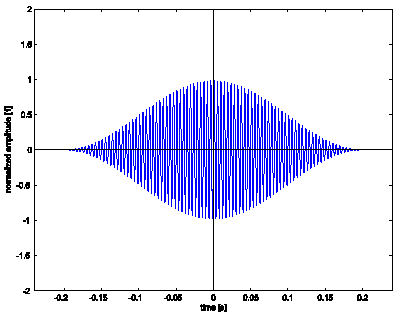
\includegraphics[width=6cm]{../NaT1/bilder/signal_energiesignal.png}
       	\end{center}

	\end{minipage}
	&
	\begin{minipage}[t]{9cm}
		\textbf{Leistungssignal} - \textit{''Dauersignal '' bspw. Trägersignal} \\
		$ E = \infty \text{ und } P < \infty$ \\
		\begin{center}
			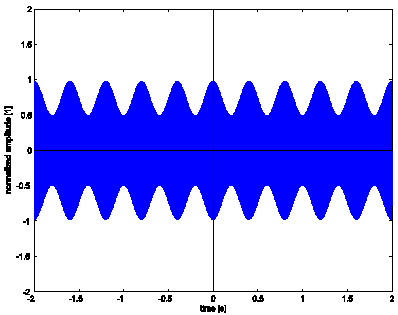
\includegraphics[width=6cm]{../NaT1/bilder/signal_leistungssignal.png}
       	\end{center}

	\end{minipage} \\

\hline

	\begin{minipage}[t]{9cm}
		\textbf{Aperiodisch} \\
		$x(t) \neq x(t + n \cdot T)$
	\end{minipage}
	&
	\begin{minipage}[t]{9cm}
		\textbf{Periodisch} \\
		$x(t) = x(t + n \cdot T) \qquad \text{ mit Periodendauer } T \text { und } n \in \mathbb{Z}$
	\end{minipage}
\\
\hline

	\begin{minipage}[t]{9cm}
		\textbf{Deterministisch} - \textit{mit vorbestimmten Verlauf} \\
		$x(t) = f(t)$
	\end{minipage}
	&
	\begin{minipage}[t]{9cm}
		\textbf{Stochastisch} - \textit{ohne vorbestimmten Verlauf} \\
		$x(t) = ?$
	\end{minipage}
\\
\hline
\end{tabular}
\newpage
\begin{tabular}[c]{ | p{9cm} | p{9cm} | }
\hline

	\begin{minipage}[t]{9cm}
		\textbf{Zeitkontinuierlich} \\
		$x(t) \text{ ist definiert } \forall t \in \mathbb{R}$
		\begin{center}
			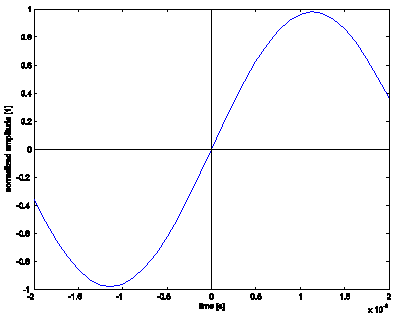
\includegraphics[width=6cm]{../NaT1/bilder/signal_zeitkontinuierlich.png}
       	\end{center}
	\end{minipage}
	&
	\begin{minipage}[t]{9cm}
		\textbf{Zeitdiskret} \\
		$x(t) \text{ nur definiert an Stellen } x(n \cdot T) $ \\
		$  \text{ mit Abtastintervall } T \text { und } n \in \mathbb{Z}$
		\begin{center}
			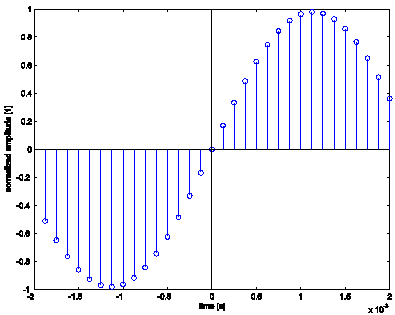
\includegraphics[width=6cm]{../NaT1/bilder/signal_zeitdiskret.png}
       	\end{center}
	\end{minipage}
\\
\hline

	\begin{minipage}[t]{9cm}
		\textbf{Amplitudenkontinuierlich}
		\begin{center}
			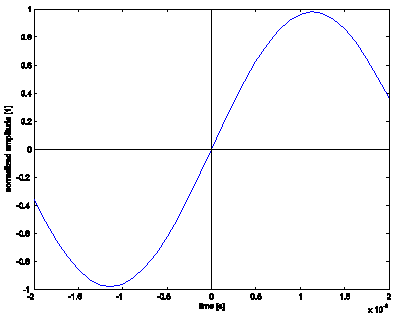
\includegraphics[width=6cm]{../NaT1/bilder/signal_amplitudenkontinuierlich.png}
       	\end{center}
	\end{minipage}
	&
	\begin{minipage}[t]{9cm}
		\textbf{Quantisiert}
		\begin{center}
			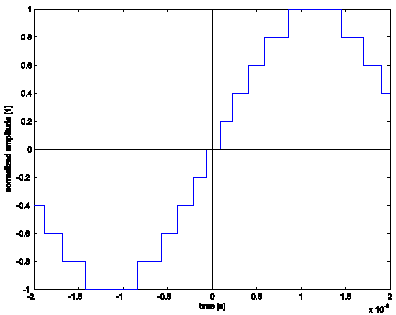
\includegraphics[width=6cm]{../NaT1/bilder/signal_quantisiert.png}
       	\end{center}
	\end{minipage}
\\
\hline

	\begin{minipage}[t]{9cm}
		\textbf{Analog} - \textit{zeit- und amplitudenkontinuierlich} \\

	\end{minipage}
	&
	\begin{minipage}[t]{9cm}
		\textbf{Digital} - \textit{zeitdiskret und quantisiert} \\

	\end{minipage}
\\
\hline
\end{tabular}
\renewcommand{\arraystretch}{1}


\skriptsection{LTI-Systeme}{25}
\begin{center}
	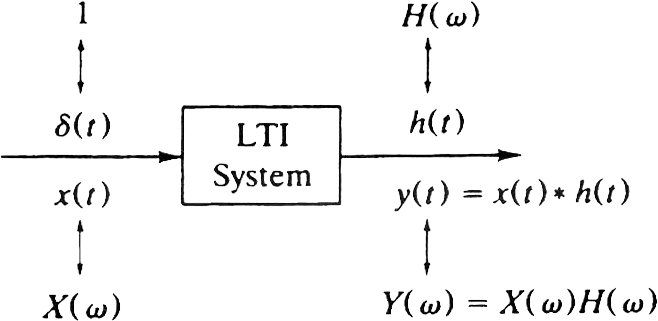
\includegraphics[width=10cm]{../NaT1/bilder/lti-system.png}
\end{center}


%\subsection{Eigenschaften von LTI-Systemen}
$ y(t) = T [ x(t)] \qquad $ Operator T erzeugt aus dem Eingangssignal $ x(t) $ das Ausgangssignal $ y(t)$. \\
\textbf{Linearität und Zeitinvarianz gelten!}

\paragraph{Kausalität} Ein System ist kausal, wenn jedes Ausgangsignal durch ein vorhergehendes Eingangsignal gebildet wird.
\\
\hrule
\subsection{Schrittfunktion - unit step}
\begin{minipage}{10cm}
	$u(t) =	\begin{cases}
	  		 0 & \text{für } t < 0 \\
	  		 \frac{1}{2} \text{(praxis)}  \text{ oder undef. (math.)} & \text{für } t = 0 \\
	  		 1 & \text{für } t > 0
	  	\end{cases}
	$
\end{minipage}
\begin{minipage}{8cm}
	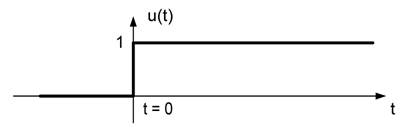
\includegraphics[width=6cm]{../NaT1/bilder/unitstep.png}
\end{minipage}


\subsection{Impulsfunktion - dirac delta function}
	\begin{minipage}{10cm}
		$\delta (t)=\begin{cases} 0 & t\ne 0\\\infty & t=0\end{cases} \qquad
		\text{und} \qquad \int\limits_{-\infty}^\infty \delta(t) \, \mathrm dt = 1 $\\
		$$\frac{du(t)}{dt}=\delta(t) \qquad
		\int\limits_{-\infty}^{\infty}\delta(t-t_0)f(t)dt=f(t_0)$$
	\end{minipage}
	\begin{minipage}{8cm}
		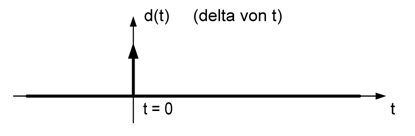
\includegraphics[width=6cm]{../NaT1/bilder/diracimpulse.png}
	\end{minipage}

\hrule
\skriptsubsection{Impulsantwort}{25-2.2B}
Siehe Signale \& Systeme Zusammenfassung.\\
%$h(t) = T[\delta(t)] \qquad $

\hrule
\skriptsubsection{Verzerrungen}{26}
\subsubsection{Amplitudenverzerrung}
Falls das Amplitudenspektrum $|H(\omega)|$ im gewünschten Frequenzband nicht konstant ist,
resultieren Amplitudenverzerrungen.

\subsubsection{Phasenverzerrung}
Falls das Phasenspektrum $\Theta_h (\omega)$ nicht linear von der Frequenz abhängig ist, resultieren
Phasenverzerrungen.\\
\hrule
\skriptsubsection{Filter}{27}
\begin{list}{$\bullet$}{\setlength{\itemsep}{0cm} \setlength{\parsep}{0cm} \setlength{\topsep}{0cm}} 
  \item Tiefpass - Lowpass Filter (LPF)
  \item Hochpass - Highpass Filter (HPF)
  \item Bandpass - Bandpass Filter (BPF)
  \item Bandsperre - Bandstop Filter (BSF)
\end{list}
\paragraph{Ideale Filter} sind nicht realisierbar, da sie akausal sind.

\skriptsubsubsection{Bandbreite}{28}
\begin{minipage}{7cm}
	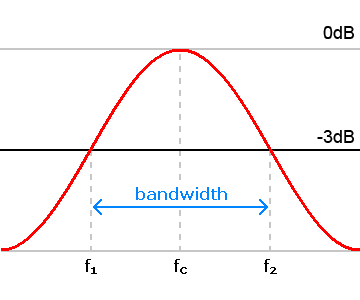
\includegraphics[width=6cm]{../NaT1/bilder/filter_bandbreite.png}
\end{minipage}
\begin{minipage}{11cm}
	Die Bandbreite ist nur für Tief- und Bandpassfilter definiert und bezieht sich auf das einseitige (reelle) Spektrum.
	\paragraph{LPF}	Die Bandbreite $W_B = 2 \pi B$ eines LPF entspricht der Frequenz, bei der $|H(\omega)|$ gegenüber $|H(0)|$ um $3 dB$ gedämpft ist
	\paragraph{BPF}	Filterbandbreite $W_B = 2 \pi B$ bei BPF entspricht der Differenz der (Kreis-) Frequenzen, bei denen Amplitudengang $|H(\omega)|$ gegenüber $|H(\omega_c)|$ um
	$3 dB$ gedämpft ist
\end{minipage}


\skriptsubsubsection{Quadraturfilter}{29} \label{lti_quadratur}
Ein Quadraturfilter ist ein Allpassfilter mit Phasendrehung um $-\frac{\pi}{2}\text{rad } (-90^\circ)$. \\
$$H(\omega) = \begin{cases}
             	e^{-j \frac{\pi}{2}} & \omega > 0 \\
             	e^{j \frac{\pi}{2}} & \omega < 0
             \end{cases} =
-j \sgn(\omega)$$

Dieses Filter ist technisch nur für einen beschränkten Bandbreitenbereich realisierbar.

\skriptsubsubsection{Hilbert Transformation}{29} \label{lti_hilbert}
Bewirkt eine $-90^\circ$ Phasendrehung des Signals $x(t)$.
$$\qquad \hat{X}(\omega) = H(\omega)X(\omega) = [-j \sgn(\omega)] X(\omega)$$















%%%%%%%%%%%%%%%%%%%%%%%%%%%%%%%%%%%%%%%%%%%%%%%%%%%%%%%%%%%%%%%%%%%%%%%%%%%%%%%%%%%%%%%%%%%%%%%%
%%%%%%%%%%%%%%%%%%%%%%%%%%%%%%%%%%%%%%%%%%%%%%%%%%%%%%%%%%%%%%%%%%%%%%%%%%%%%%%%%%%%%%%%%%%%%%%%
\newpage
\skriptsection{AM (Amplitudenmodulation)}{43}
Bei der Amplitudenmodulation ist die Amplitude des Trägersignals $A(t)$ linear von der dem
Nachrichtensignal $m(t)$ abhängig.

$$ x_c(t) = A(t) \cos(w_c t) $$




\skriptsubsection{DSB(-SC): Doppelseitenband (Double-Sideband)-AM}{44}
Bei der Doppelseitenband-Amplitudenmodulation ist das untere Seitenband (Lower
Sideband) sowie das
obere Seitenband (Upper Sideband) präsent. Da der Träger im Spektrum nicht
präsent ist, ist bei dieser Art von AM auch von \textbf{DSB-SC (Double-Sideband Suppressed Carrier)} die Rede. \\ 
Die \textbf{Bandbreite} berechnet sich dadurch wie folgt: $ \qquad W_B = 2 w_{\omega}$

\subsubsection{Modulation}
\begin{minipage}[c][2.7cm][t]{6.5cm}
    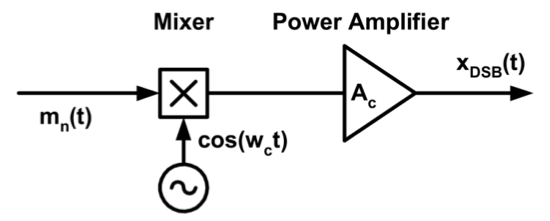
\includegraphics[width=6cm]{../NaT1/bilder/am_dsb_modulation.png}
\end{minipage}
\begin{minipage}[c][2.7cm][t]{11.5cm}
Bei der Doppelseitenband AM wird das Nachrichtensignal mit dem sinusförmigen Trägersignal
multipliziert, wodruch sich dank dem Modulationssatz folgendes Spektrum ergibt. \\
$$ x_{DSB}(t) =
m(t) \cos(w_c t) \quad \laplace \quad X_{DSB} = \frac{1}{2}M(\omega - \omega_c) + \frac{1}{2}M(\omega + \omega_c)$$
\end{minipage}

\begin{minipage}[t]{9.5cm}
    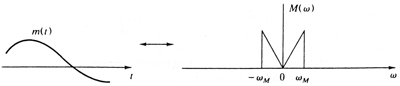
\includegraphics[width=9cm]{../NaT1/bilder/am_dsb_nachrichtensignal.png}
\end{minipage}
\begin{minipage}[t]{9cm}
    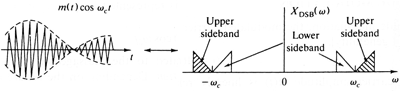
\includegraphics[width=9cm]{../NaT1/bilder/am_dsb_spektrum.png}
\end{minipage}

\subsubsection{Demodulation} 
\label{am_dsb_modulation}
\begin{minipage}[t][2.3cm][c]{6.5cm}
    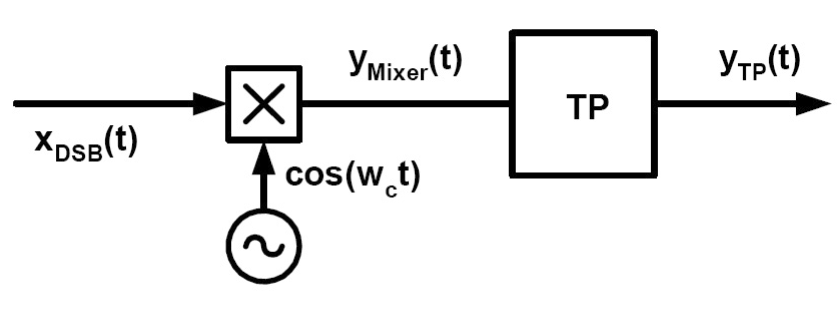
\includegraphics[width=6cm]{../NaT1/bilder/am_dsb_demodulation.png}
\end{minipage}
\begin{minipage}[t][2.3cm][c]{11.5cm}
	Das DSB-Signal wird mit einem sogenannten \textbf{synchronen Demodulator} oder \textbf{koharänten
	Demodulator} zurückgewonnen. Hierbei wird das DSB-Signal mit dem lokalen Träger
	multipliziert und anschliessend das Nachrichtensignal mittels einem Tiefpassfilter rausgefiltert.
	\\ Weicht die Frequenz oder die Phase des lokalen Trägers von deren, des ursprünglichen Trägers ab, 
	so ergeben sich Abschwächungen im demodulierten Nachrichtensignal.
\end{minipage}

\paragraph{Auswirkungen einer Phasenabweichung um $\phi$:} $y_{TP}(t) = \frac{1}{2}
m(t) \cos(-\phi)= \frac{1}{2} m(t) \cos(\phi) $
\paragraph{Auswirkungen einer Frequenzabweichung um $\Delta \omega$:} $y_{TP}(t) =
\frac{1}{2} m(t) \cos(\Delta \omega t)$\\


\hrule
\skriptsubsection{AM: Gewöhnliche(Ordinary)-AM}{45}
Die gewöhnliche AM wird generiert, indem man dem DSB-Signal ein grosses Trägersignal dazuaddiert.

\subsubsection{Modulation}

$$x_{AM}(t) = A_C (1 + \mu \cdot m(t)) \cos(\omega_c t)
	\quad \laplace \quad X_{AM}(\omega) = \frac{1}{2}M(\omega - \omega_c) + \frac{1}{2}M(\omega + \omega_c)
	+ \pi A [\delta (\omega - \omega_c) + \delta (\omega + \omega_c))]$$

\begin{minipage}[]{9cm}
	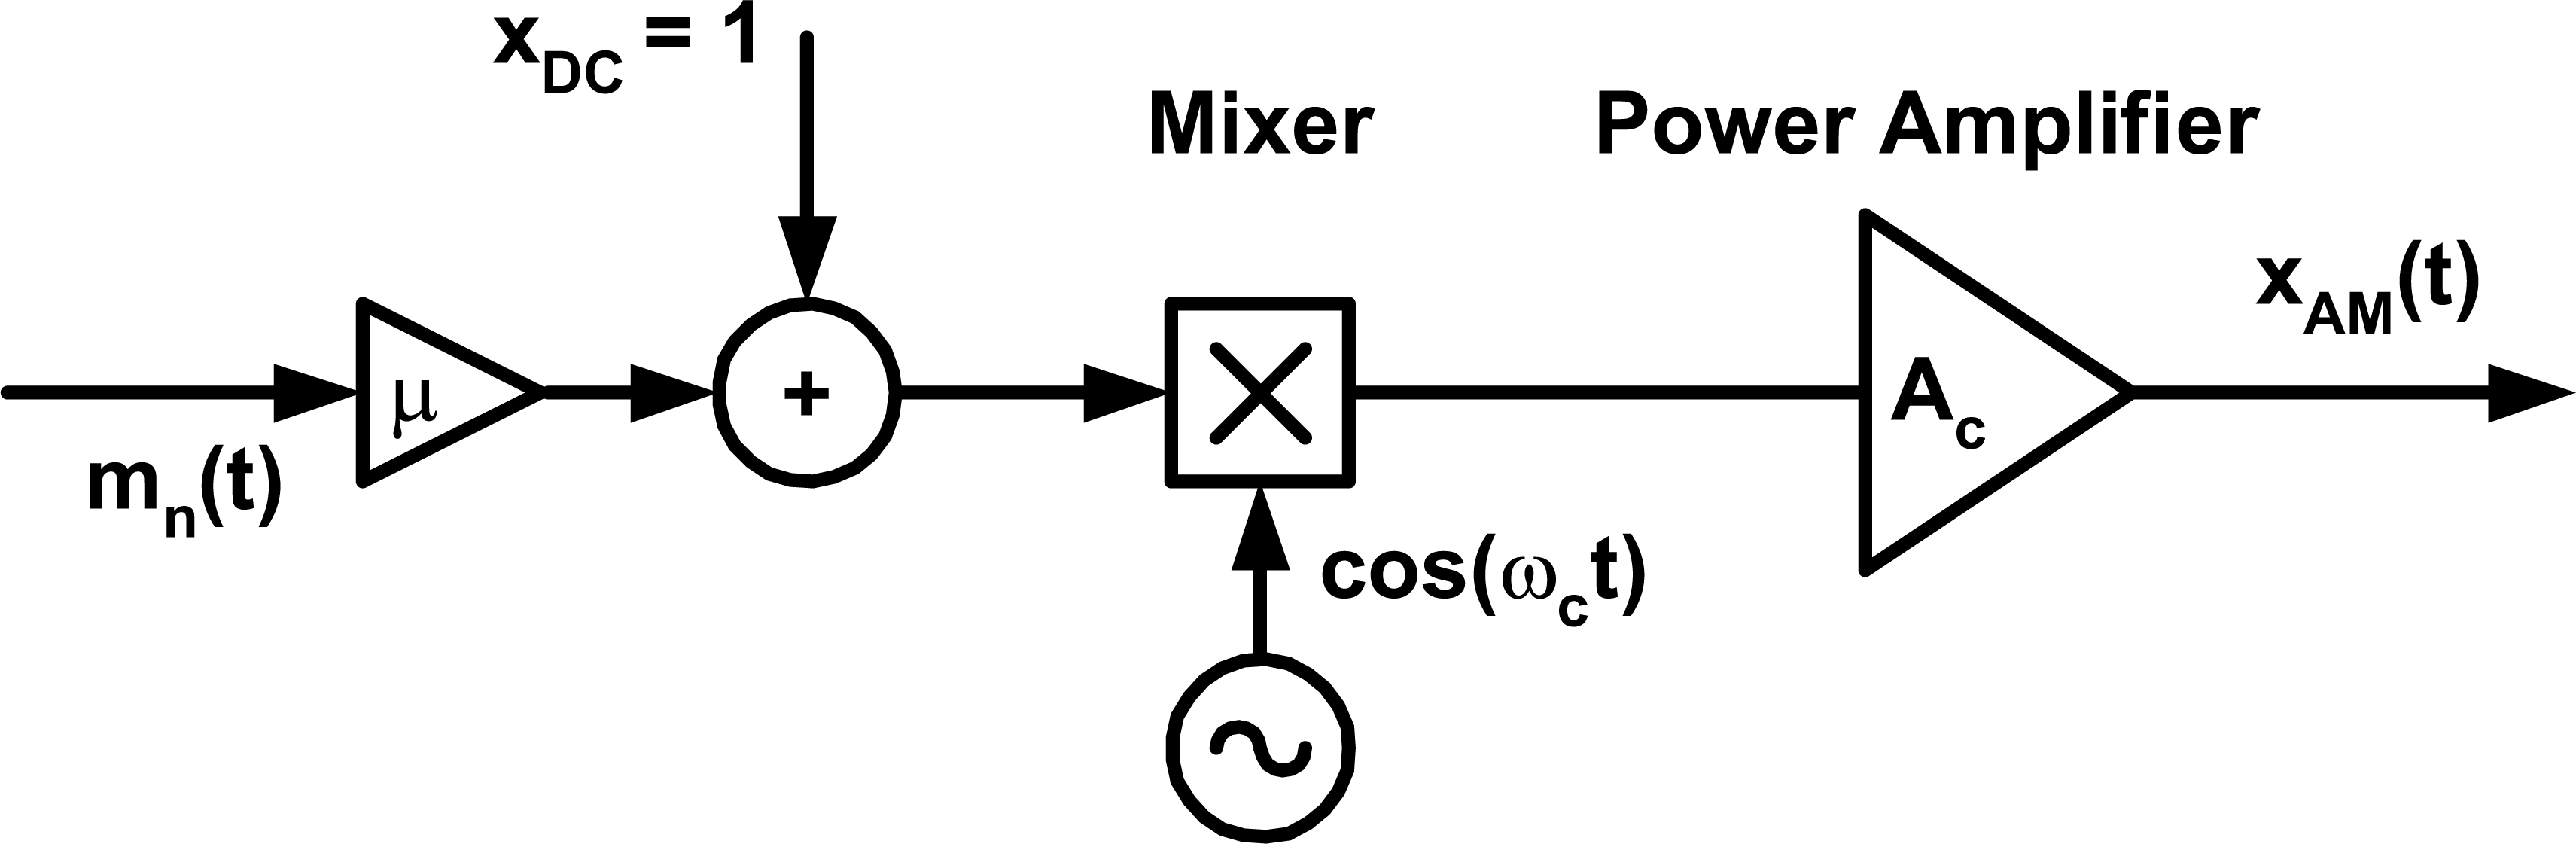
\includegraphics[width=9cm]{../NaT1/bilder/am_oam_modulation.png}
\end{minipage}
\begin{minipage}[]{9cm}
    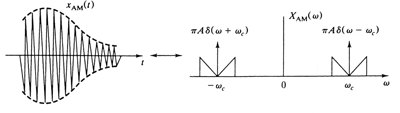
\includegraphics[width=9cm]{../NaT1/bilder/am_oam_spektrum.png}
\end{minipage}\\
Die Bandbreite bleibt gleich wie bei DSB-AM, jedoch befindet sich nun ein grosser Teil der
Signalleistung im Träger. \\
Diese Art von AM hat sich v.a. in füheren Zeiten durchgesetzt, weil die Demodulation mit sehr
wenig Aufwand realisiert werden kann. 

\subsubsection{Demodulation}
\paragraph{Mit Enveloppen Detektor}
Der Enveloppen Detektor braucht nur drei Bauteile, der Schaltungsaufwand ist also
sehr gering.\\
\begin{center}	
      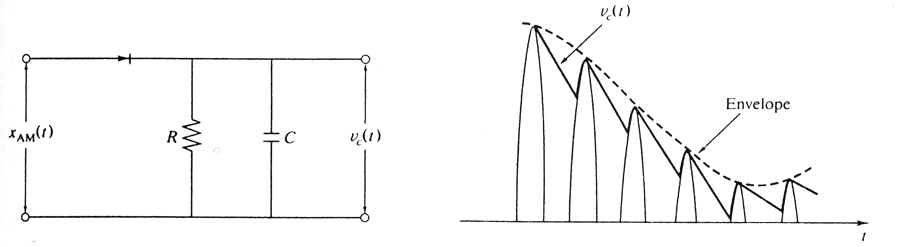
\includegraphics[width=14cm]{../NaT1/bilder/am_oam_enveloppeDetektor.png}
\end{center}
Damit der Envelope Detektor korrekt funktioniert müssen R und C korrekt gewählt werden, es gilt:
$RC \leq \frac{\sqrt{1 - \mu^2}}{\omega_m \mu}$ \\
In der Praxis genügt jedoch das Erfüllen der Bedingung $\frac{1}{\omega_c} \ll \frac{1}{W_M}$,
wobei es sich bei $W_M$ um die Bandbreite des Nachrichtensignals handelt. 

\paragraph{Mit kohärentem (synchronen) Demodulator}
Ordinary AM kann auch mit dem kohärenten Demodulator demoduliert werden
\verweis{am_dsb_modulation}{}:
$y(t) = \frac12 (A + m(t)) = \frac12 m(t) + \frac12 A$ mit nachfolgendem
seriellem Kondensator (Hochpass).


\skriptsubsubsection{Modulationsindex}{46}
Der Modulationsindex $\mu$ ist für AM wie folgt definiert.
$$\mu = \frac{|min\{m(t)\}|}{A_c} = \frac{A_m}{A_c} $$
Um eine Demodulation mit dem Envelope-Detektor zu ermöglichen, muss die Bedingung 
\textbf{$\mu \ll 1$} erfüllt sein. \\
Ist dies nicht der Fall (\textbf{$\mu > 1$}) so spricht man von einer \textbf{Übermodulation} oder
einem  \textbf{übermodulierten Träger}, was in einer Envelope-Verzerrung resultiert. \\
Anbei zwei Fälle zur Veranschaulichung dieser Problematik: Links ($\mu \ll 1$), Rechts ($\mu > 1
\rightarrow $ Übermodulation).

\begin{minipage}[t][2.3cm][c]{9.5cm}
	\begin{center}
      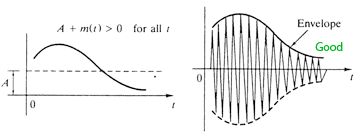
\includegraphics[width=8cm]{../NaT1/bilder/am_oam_enveloppeGood.png}
	\end{center}
\end{minipage}
\begin{minipage}[t][2.3cm][c]{9.5cm}
    \begin{center}
    	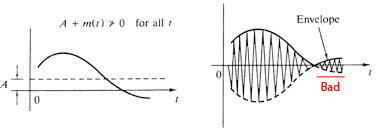
\includegraphics[width=8cm]{../NaT1/bilder/am_oam_enveloppeBad.png}
	\end{center}
\end{minipage}

\skriptsubsubsection{Effizienz / Wirkungsgrad}{55-3.4}
Unter der Effizienz $ \eta $ der gewöhnlichen AM versteht man das Verhältnis von der Signalleistung
$P_s$ der beiden Seitenbänder zur Gesamtleistung $P_t$ des AM-Signals.

$$ P_c = \frac{A_c^2}{2} \quad \text{und} \quad P_t = \frac{A_c^2}{2} + \frac{\mu^2 A_c^2}{4}
\quad \Longrightarrow \quad \eta = \frac{P_s}{P_t} = \frac{P_t - P_c}{P_t} = \frac{\mu^2}{2+\mu^2} $$

Die maximale Effizienz (bei $\mu = 100\% $) beträgt nur gerade $ \eta = 33\% $. Bei $\mu = 50\% $
sind es noch bescheidene $\eta = 11.1\% $.


\newpage
\skriptsubsection{SSB: Einseitenband (Single-Sideband)-AM}{47}
Sowohl Gewöhnliche AM als auch DSB verschwenden Bandbreite, weil diese immer beide Seitenbänder
übermitteln. \\
Ist dies nicht der Fall - wird also \textbf{nur ein Seitenband} übertragen - so spricht man von
Einseitenband-AM. Deren Vorteil liegt in der Reduktion der Bandbreite, was aber auch den Nachteil
- Die Komplexität der Implementation - mit sich bringt.

\subsubsection{Modulation}
\textbf{Phasenverschiebung \formelbuch{59-3.8}}  \\
\begin{minipage}[t][3.7cm][c]{7.5cm}
    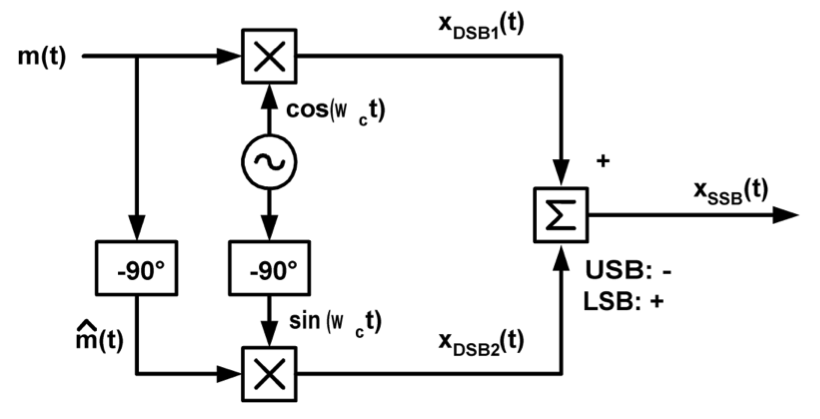
\includegraphics[width=7cm]{../NaT1/bilder/am_ssb_modulationPhasenshifter.png}
\end{minipage}
\begin{minipage}[t][3.7cm][c]{10.5cm}	
	Des weiteren bieter sich die Möglichkeit ein SSB-Signal mit Hilfe von 
	$ - 90^{\circ} $-Phasenschiebern zu generieren, {\small siehe
	\ref{lti_quadratur} Quadraturfilter (S. \pageref{lti_quadratur}) \&
	\ref{lti_hilbert} Hilbertransformation (S. \pageref{lti_hilbert})}.\\
	Die Amplitude des SSB-Signals ist im Spektrum \textbf{gleich hoch} wie die des
	Nachrichtensignals.\\ 
	$+$: Lower Sideband; \qquad $-$: Upper Sideband
\end{minipage}

\textbf{Frequenzdiskriminierung} \\
\begin{minipage}[t][2cm][c]{5.5cm}
    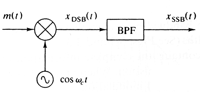
\includegraphics[width=5cm]{../NaT1/bilder/am_ssb_modulationFilter.png}
\end{minipage}
\begin{minipage}[t][2cm][c]{12.5cm}	
	Hierbei wird ein DSB-Signal mit einem Hoch- oder Tiefpass gefiltert, sodass ein SSB-Signal
	resultiert. Diese Methode ist in der \textbf{Praxis unüblich}, da sehr steile Filter benötigt
	werden.\\
	Die Amplitude des SSB-Signals ist im Spektrum \textbf{halb so hoch} wie die des
	Nachrichtensignals.
\end{minipage}

\subsubsection{Demodulation}
Diese erfolgt wie bei DSB-AM \verweis{am_dsb_modulation}{Modulation DSB-AM}.\\

\hrule
\skriptsubsection{VSB: Restseitenband (Vestigial-Sideband)-AM)}{49}
\subsubsection{Modulation}
\begin{minipage}[t][2.2cm][c]{5.5cm}
    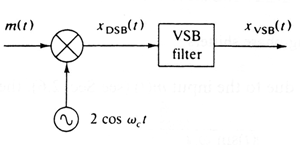
\includegraphics[width=5cm]{../NaT1/bilder/am_vsb_modulator.png}
    %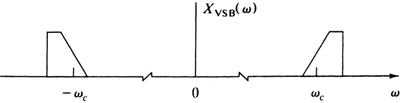
\includegraphics[width=7cm]{../NaT1/bilder/am_vsb_spektrum.png}
\end{minipage}
\begin{minipage}[t][2.2cm][c]{12.5cm}	
Restseitenband-AM ist sozusagen die praktische Realisierung der Frequenzdiskriminierungsmethode bei
SSB. Es wird ein DSB-Signal mit einem Restseitenbandfilter (sideband-shaping filter) gefiltert,
wodurch schlussendlich das VSB-Singal resultiert mit etwa 1.25-facher Bandbreite von SSB.
$ \qquad  W_{VSB} \approx 1.25 \cdot W_{SSB} $
\end{minipage}
\begin{center}
    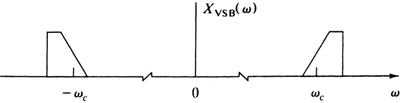
\includegraphics[width=8cm]{../NaT1/bilder/am_vsb_spektrum.png}
\end{center}

\subsubsection{Demodulation}
Auch diese Art von AM kann mit einem kohärenten Demodulator demoduliert
werden \verweis{am_dsb_modulation}{Modulation DSB-AM}.\\
Für eine verzerrungsfreie Demodulation ist erforderlich, dass $H(\omega +
\omega_c) + H(\omega - \omega_c) = const$ für $|\omega| \leq |\omega_m|_{max}$.

\newpage
\skriptsubsection{QAM: Quadratur(Quadrature)-AM}{64-3.15}
Hierbei werden zwei orthogonale Träger ($\sin, \cos$) verwendet, sodass zwei Nachrichtensignale
zusammen übertragen werden können. Dies ist zwar technisch aufwendiger, jedoch wird die Bandbreite
doppelt genutzt. \\
Bei der Demodulation muss darauf geachtet werden, dass der Demodulator synchronisiert ist. Ist dies
nicht der Fall, so kann sich bei grösserer Phasenabweichung das andere Nachrichtensignal
``einschleichen''.
\begin{center}
    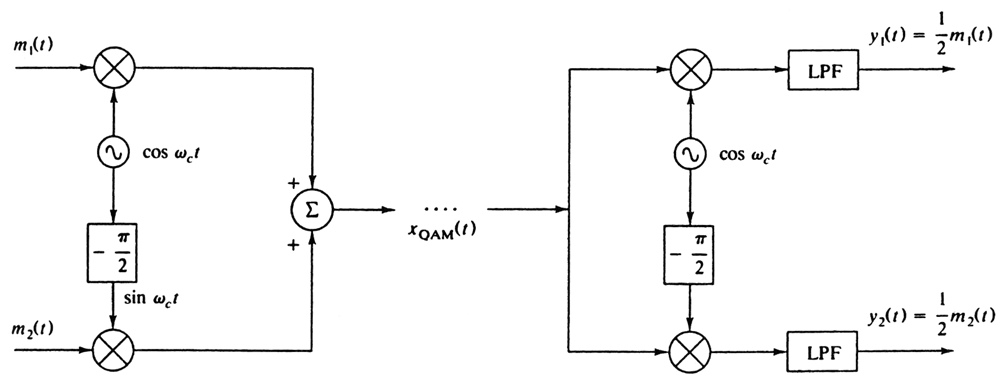
\includegraphics[width=14cm]{../NaT1/bilder/am_qam_modulatorDemodulator.png}
\end{center}











\hrule
%%%%%%%%%%%%%%%%%%%%%%%%%%%%%%%%%%%%%%%%%%%%%%%%%%%%%%%%%%%%%%%%%%%%%%%%%%%%%%%%%%%%%%%%%%%%%%%
%%%%%%%%%%%%%%%%%%%%%%%%%%%%%%%%%%%%%%%%%%%%%%%%%%%%%%%%%%%%%%%%%%%%%%%%%%%%%%%%%%%%%%%%%%%%%%%
\skriptsection{Winkelmodulation (FM/PM)}{68}
Obwohl Winkel- und Frequenzmodulation - im Vergleich zu AM - komplexer ist und mehr Bandbreite
benötigt hat es einen erheblichen Vorteil, welcher die vorhin genannten Nachteile kompensiert.
Nämlich ist die \textbf{Störanfälligkeit} und das \textbf{Rauschen} kleiner als bei AM. \\
\\
Die Grundlage bietet der sinusförmige Träger, wessen Phase oder Frequenz je nach Amplitude des 
Nachrichtensignals moduliert wird.

$$\boxed{ x_c(t) = A \cos(w_c t + \phi(t)) = A \cos(\theta(t)) }$$

\begin{center}
\renewcommand{\arraystretch}{2}
\begin{tabular}{|p{8cm}|p{8cm}|}
	\hline
	\textbf{PM} &	\textbf{FM}\\
	\hline
	$\phi(t) = k_p m(t)$ &
	$ \frac{d \phi(t)}{dt} = k_f m(t) \Rightarrow \phi(t) = k_f \int\limits_{t_0}^{t} m(\lambda)
	d\lambda + \phi(t_0)$\\
	$x_{PM}(t) = A \cos[w_c t + k_p m(t)]$ &
	$x_{FM}(t) = A \cos[w_c t + k_f \int\limits_{- \infty}^{t} m(\lambda)
	d\lambda]$\\
	\hline
	$k_p=$ Phasenhubkonstante $[rad]$ & $k_f=$ Frequenzhubkonstante
	$[\frac{rad}{s}]$\\
	\hline
\end{tabular} 
\renewcommand{\arraystretch}{1}
\end{center}

\hrule
\subsection{Momentanfrequenz, Frequenzabweichung}
\begin{minipage}[t]{10cm}
	$$ w_i = \frac{d \theta(t)}{dt} = w_c + \frac{d \phi(t)}{dt} $$
	$$ \Delta \omega = \left| \omega_i - \omega_c \right|_{max} $$
\end{minipage}
\begin{minipage}[t]{8cm}
	$\omega_i$ Momentanfrequenz, $[\omega_i] = \frac{rad}{s}$ \\
	$\omega_c$ Trägerfrequenz, $[\omega_c] = \frac{rad}{s}$ \\
	$\Delta \omega$ maximale Frequenzabweichung, $[\Delta \omega] = \frac{rad}{s}$ \\
	$\theta(t)$ momentane Phasenabweichung, $[\theta(t)] = \frac{rad}{s}$\\
\end{minipage}

\hrule
\skriptsubsection{Klein- und Grosshub}{70-4.5}
Abhängig von der maximalen Phasenabeweichung sind zwei verschiedene Arten von Winkelmodulationnen zu
unterscheiden. \\

\begin{tabular}{llll}
\textbf{Kleinhub - NB (Narrowband)} 
	& $|\phi(t)|_{max} < 0.2$ 
	& $\Leftrightarrow \quad \beta < 0.2$
	& $\Leftrightarrow \quad D < 0.2$ \\

\textbf{Grosshub - WB (Wideband)}
 & $|\phi(t)|_{max} \gg 1$
 & $\Leftrightarrow \quad \beta \gg 1$
 & $\Leftrightarrow \quad D \gg 1$ \\

\end{tabular}
 
\newpage

\skriptsubsection{Einton (Sinusförmige)-Modulation (Sinusoidal
Modulation)}{71-4.6}

\subsubsection{Modulationsindex (Modulation Index)}
\begin{minipage}[t][0.7cm][c]{10cm}

$ m(t) = \begin{cases}
          	a_m \sin(\omega_m t)  & \textbf{PM}\\
          	a_m \cos(\omega_m t)  & \textbf{FM}
          \end{cases}  
\qquad
\beta = \dfrac{\Delta \omega}{\omega_m} =
\begin{cases}
	k_p a_m & \textbf{PM}  \\
	\frac{k_f a_m}{\omega m} & \textbf{FM}
\end{cases} 
$
\end{minipage}
\begin{minipage}[t][0.7cm][c]{8cm}
	$\beta$ Modulationsindex (max. Phasenabw.), $[\beta] = rad$ \\
	$a_m$ Amplitude des Nachrichtensignals, $[a_m] = 1$ %\\
	%$k_f$ Frequenzabweichungskonstante, $[k_f] = 1$ \\
	%$k_f$ Phasenabweichungskonstante, $[k_p] = 1$
\end{minipage}

\subsubsection{Spektrum}
$$x_c(t) = A \cos(\omega_c t + \beta \sin(\omega_m t)) \quad \Rightarrow \quad 
x_c(t) = A \sum\limits_{n=-\infty}^{\infty} J_n(\beta) \cos((\omega_c + n \omega_m)t)$$
%%\paragraph{Bessel Funktion}
\textbf{$J_n(\beta)$} ist die \textbf{Bessel Funktion erster Art $n$-ter Ordnung} (Schaum
S. 323f). Das Spektrum besteht aus dem Trägersignal plus einer unendlichen Anzahl Spektrallinien,
wobei $J_n(\beta)$ sehr klein ist für grosse $n$. \\
Für ($\beta \ll 1$, Kleinhub) sind nur $J_0$, $J_1$ und $ J_{-1}$ relevant. Bei ($\beta \gg 1$,
Grosshub) existieren jedoch einige signifikante Seitenbänder.
%%TODO bessel function

\subsubsection{Bandbreite}
Mit der Bedingung $J_n(\beta) \approx 0, \,\forall (n > \beta + 1)$ kann die Bandbreite approximativ
berechnet werden. 98\% der durschnittlichen Signalleistung sind in diesem
Frequenzspektrum angesiedelt. 

\begin{center}
$W_B \approx 2(\beta + 1) \omega_m = 
	\begin{cases}
  		2 \omega_m (k_p a_m + 1) & \textbf{PM},\, W_B \sim \omega_m \\
  		2(k_f a_m + \omega_m) & \textbf{FM},\, W_B \nsim \omega_m \end{cases} \qquad
  		\qquad \qquad \beta < 0.2 \text{ (NB)}: \quad W_{B} \approx 2 \omega_m
$
\end{center}

\subsubsection{Leistung \formelbuch{78-4.6}}
$$P = \frac12 A_C^2$$
\hrule


\subsection{Willkürliche-Modulation (Arbitrary Modulation) \formelbuch{72-4.7B}}
Anstelle von $\beta$ verwenden wir für willkürliche Nachrichtensignale $D$ für die
Phasenabweichung.\\ 
\begin{minipage}[t][2.7cm][c]{10cm}
	$$ D = \frac{\Delta \omega}{W_M} $$	
$$W_B \approx 2(D + 1) W_M \qquad \qquad 
	\textbf{NB}(\forall (D \ll 1)): \quad W_{B} = 2 W_M $$
 $$ \textbf{WB} (\forall (D \gg 1)): W_{PM} = 2 \Delta \omega \text{(prop. $W_M$)};
 \quad W_{FM} = 2 \Delta \omega \text{(const.)} $$
\end{minipage} \hspace{0.6cm}
\begin{minipage}[t][2.7cm][c]{8cm} 
	$D$ Modulationsindex = max. Phasenabw., $[D] = rad$ \\
	$W_M$ Bandbreite des Nachrichtensignals \\
	$\Delta \omega$ Frequenzabweichung \\
	$W_B,W_{FM},W_{PM}$ Bandbreite des winkelmodulierten Signals
\end{minipage} \\
Bei Grosshub-FM bleibt die resultierende Bandbreite $W_{FM}$ bei ändernder Nachrichtenbandbreite
$W_M$ gleich. Bei Grosshub-PM ändert sich diese Bandbreite$W_{PM}$ jedoch proportional zur
Nachrichtenbandbreite $W_M$.\\

\hrule
\subsection{Modulationsarten}
Auch bei der Modulation muss zwischen Klein- und Grosshub FM/PM unterschieden werden.

%pm_nbpm_modulator.png fm_nbfm_modulator.png

\skriptsubsubsection{Kleinhub Modulation}{72-4.8A}
Aus der trigonometrische Gleichung ($\cos(\beta + \alpha) = \cos(\alpha) \cdot \cos(\beta) -
\sin(\alpha) \cdot \sin(\beta)$ mit $\cos(\alpha) \approx 1, \sin(\alpha) \approx \alpha$) ergibt
sich: \\
$$\cos(\beta) - \alpha \cdot \sin(\beta) \quad \Rightarrow \quad \cos(\omega_c t + k_p \cdot m(t))
= \cos(\omega_c t) - k_p \cdot m(t) \sin(\omega_c t)$$

\begin{minipage}[t][3cm][c]{9cm}	
	\begin{center}
  		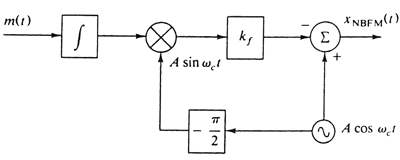
\includegraphics[height=2.8cm]{../NaT1/bilder/fm_nbfm_modulator.png} \\
  		\textbf{Kleinhub-FM Modulator}
	\end{center}
\end{minipage}
\begin{minipage}[t][3cm][c]{9cm} 
	\begin{center}
		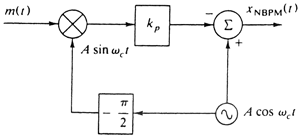
\includegraphics[height=2.8cm]{../NaT1/bilder/fm_nbpm_modulator.png} \\ 
  		\textbf{Kleinhub-PM Modulator}
	\end{center}
\end{minipage}

\skriptsubsubsection{Indirekte Grosshub Modulation}{73-4.8B1}
\begin{minipage}[t][3cm][c]{10cm}	
	Bei dieser Methode wir zuerst ein Kleinhub-Signal erzeugt und dann mittels einem
	\textbf{Frequenzmultiplikator} in ein Grosshub-Signal gewandelt.
	$$ x(t) = A \cos[\omega_c t + \Phi(t)] \quad \Rightarrow \quad y(t) = A \cos[n \omega _c t + n
	\Phi(t)]$$ Frequenzmultiplikation ist realisierbar mit nicht-linearen Bauteilen (Diode, Transistor,
	etc.).
\end{minipage}
\begin{minipage}[t][3cm][c]{8.5cm} 
	\begin{center}
		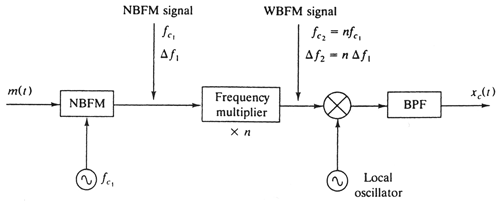
\includegraphics[height=3.4cm]{../NaT1/bilder/fm_nbfm2wbfmConverter.png}
	\end{center}
\end{minipage}

\skriptsubsubsection{Direkte Grosshub Modulation}{74-4.8B2}
Dank der spannungsabhängigen Sperrschichtkapazität von Dioden (Varicap - Kapazitätsdiode,
Dioden-Varaktor, MOS-Varaktor) ist es möglich spannungsabhängige Oszillatoren zu entwickeln. Diese \textbf{VCOs
(Voltage Controlled Oscialltor)} können dann direkt ein Grosshub PM/FM Signal
erzeugen.\\

\hrule
\subsection{Demodulation}
Die Demodulation von FM benötigt ein System, welches eine Ausgangsspannung proportional zur
momentanen Frequenzabweichung erzeugt, solch ein System nennt man Frequenzdiskriminator. \\
Auch PM kann so einfach demoduliert werden, indem am Ausgang des FM-Demodulators noch ein
Integrator nachgeschalter wird.

\subsubsection{Frequenzdiskriminator}
\begin{minipage}[t][3cm][c]{6cm}	
	\begin{center}
  		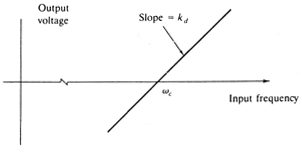
\includegraphics[height=2.8cm]{../NaT1/bilder/fm_pm_frequenzdiskriminatorAmplitudengang.png} \\
  		\textbf{Idealer Frequenzdiskriminator}
	\end{center}
\end{minipage}
\begin{minipage}[t][3cm][c]{6cm} 
	Praktisch wird der Frequenzdiskriminator durch ein Differentiator mit nachgeschaltetem
	Envelope-Detektor realisiert.
\end{minipage}
\begin{minipage}[t][3cm][c]{6cm} 
	\begin{center}
		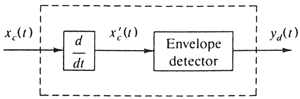
\includegraphics[width=5cm]{../NaT1/bilder/fm_pm_frequenzdiskriminatorRealisierung.png} \\ 
  		%\textbf{}
	\end{center}
\end{minipage}

\subsubsection{PLL - Phase-Locked Loop}
Bei einem PLL handelt es sich um einen phasengekoppelten Regelkreis. Dieser vergleicht die
aktuelle Frequenz eines internen Oszillators (VCO) mit einer Referenzfrequenz. Sollte die
interne Frequenz von der Referenzfrequenz abweichen, wird diese nachgeregelt. \\
Aus der Steuerspannung für den internen Oszillator resultiert genau die Frequenzabweichung und
somit auch das ursprünglich FM-modulierte Nachrichtensignal.\\

\hrule
\subsection{UKW Radio}
Das UKW Signal besteht primär aus zwei Audiosignalen: Dem Summen- (L+R) und dem Differenzsignal (L-R).
Somit kann bei schlechtem Empfang nur Mono (L+R) und bei gutem Empfang Stereo (L/R) gehört werden. \\
Zur Synchronisation mit dem Demodulator dient der 19kHz Pilot Ton. \\
Mit RDS (Radio Data System) werden Digitale Daten wie z.B. Senderinformationen (Sendername, Uhrzeit,
\ldots) mit einer Datenrate von 1187.5 bit/s übertragen. \\
\begin{minipage}{9cm}
	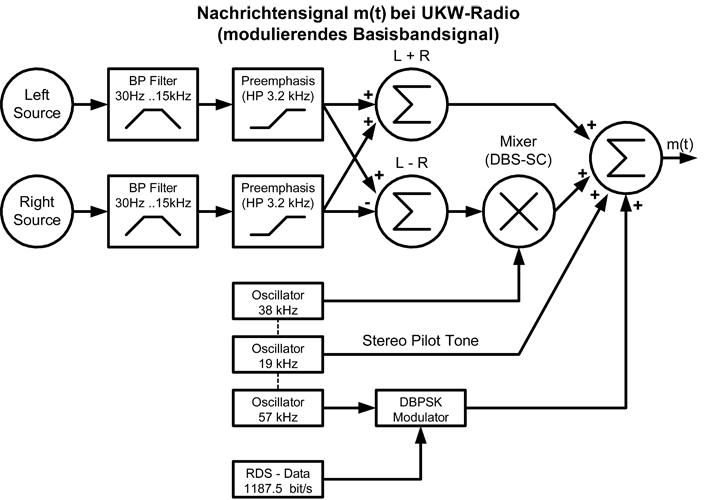
\includegraphics[width=7cm]{../NaT1/bilder/ukw_blockdiagramm.png}
\end{minipage}
\begin{minipage}{9cm} 
	\textbf{Spektrum des UKW Nachrichtensignals} \\ \\
    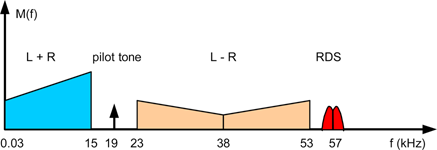
\includegraphics[width=8cm]{../NaT1/bilder/ukw_spektrum.png}
\end{minipage}

 






 
 
 


%%%%%%%%%%%%%%%%%%%%%%%%%%%%%%%%%%%%%%%%%%%%%%%%%%%%%%%%%%%%%%%%%%%%%%%%%%%%%%%%%%%%%%%%%%%%%%%
%%%%%%%%%%%%%%%%%%%%%%%%%%%%%%%%%%%%%%%%%%%%%%%%%%%%%%%%%%%%%%%%%%%%%%%%%%%%%%%%%%%%%%%%%%%%%%%
\newpage
\section{Multiplexingverfahren} \label{multiplex}


\begin{itemize}
  \item Zeitmultiplex - Time Division Multiple Access (TDMA), \textit{GSM, DECT, ISDN}
  \item Frequenzmultiplex - Frequency Division Multiple Access (FDMA), \textit{UKW-Radio}
  \item Codemultiplex - Code Division Multiple Access (CDMA), \textit{UMTS, GPS}
  \item Raummultiplex - Space Division Multiple Access (SDMA), \textit{Zellen der GSM-Basisstationen}
\end{itemize}

\skriptsubsection{FDM - Frequenzmultiplex (Frequency-Division Multiplexing)}{52}
Mit dieser Technik werden mehrer Modulierte Signale über ein Kanal gesendet. Die einzelnen
Trägerfrequenzen sind so ausgelegt, dass sich die Signale im gemeinsamen Kanal nicht überlagern und
kein Übersprechen stattfindet. Somit können die Nachrichtensignale unabhängig von den anderen
wieder demoduliert werden.
\begin{center}
    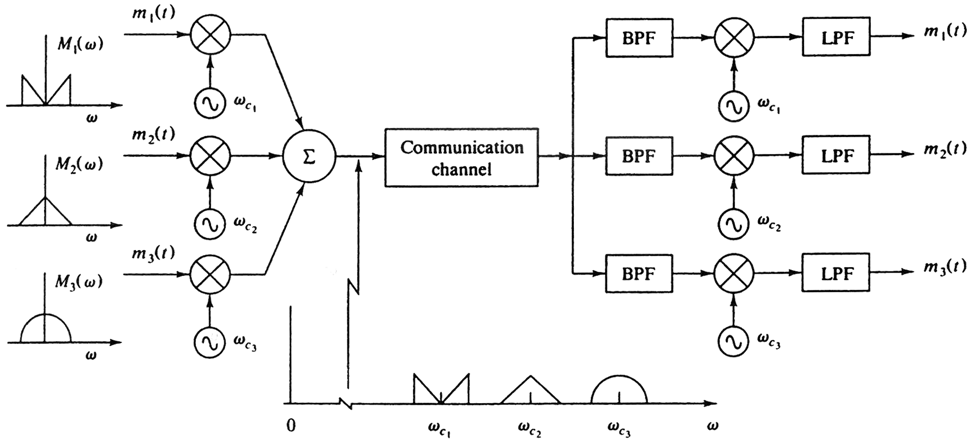
\includegraphics[width=14cm]{../NaT1/bilder/multiplex_fdm_blockdiagramm.png}
\end{center}

\skriptsubsection{TDM - Zeitmultiplex (Time-Division Multiplexing)}{100}
Bei TDM werden mehrere Nachrichtensignale über einen Kommunikationskanal gesendet, indem jedes
einzelne Signal jeweils nur zu bestimmten Zeitintervallen gesendet wird. Diese Umschaltung erfolgt
durch einen sogenannten Commutator. \\
Zeitmultiplex ist das wichtigste Mutiplexingverfahren für
Sprachübertragung inm Telekommunikationsnetz.
\begin{center}
    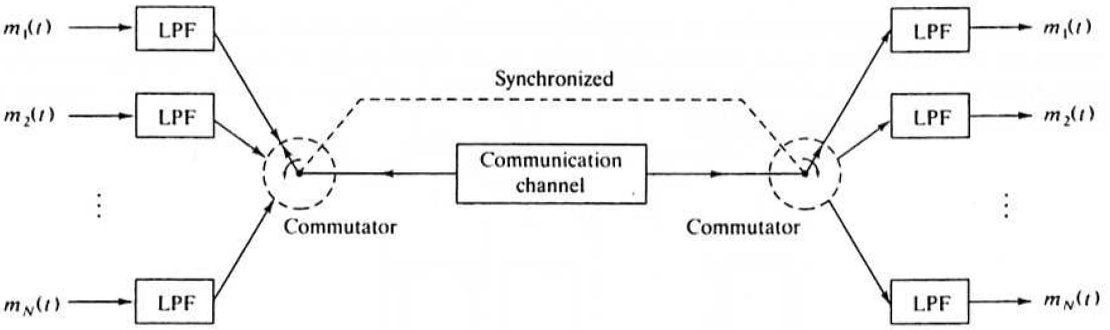
\includegraphics[width=14cm]{../NaT1/bilder/multiplex_tdm_blockdiagramm.png} \\
    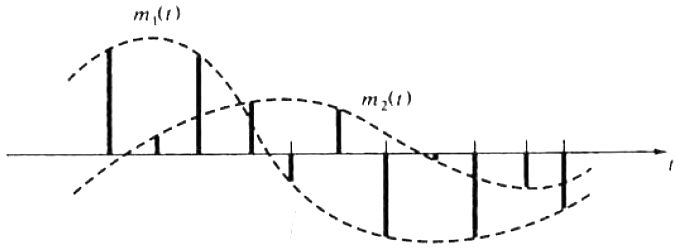
\includegraphics[height=3cm]{../NaT1/bilder/multiplex_tdm_zeitdiagramm.png}     
\end{center}











%%%%%%%%%%%%%%%%%%%%%%%%%%%%%%%%%%%%%%%%%%%%%%%%%%%%%%%%%%%%%%%%%%%%%%%%%%%%%%%%%%%%%%%%%%%%%%%%
%%%%%%%%%%%%%%%%%%%%%%%%%%%%%%%%%%%%%%%%%%%%%%%%%%%%%%%%%%%%%%%%%%%%%%%%%%%%%%%%%%%%%%%%%%%%%%%%
\newpage
\skriptsection{Digitale Uebermittlung analoger Signale}{90}

%\subsection{PCM - Pulse Code Modulation}
\begin{center}
	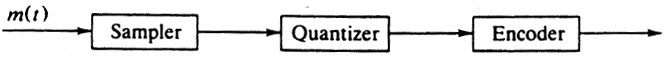
\includegraphics[width=10cm]{../NaT1/bilder/dig_pcm_blockdiagramm.png}
\end{center}
\begin{enumerate}
  \item Abtastung(Sampler): Zeitdiskretisierung 
  \item Quantisierung(Quantizer): Amplitudendiskretisierung
  \item Encoder(Codierung)
\end{enumerate}

Einige Vorteile der Digitalisierung: $\approx$ 100\% Störungsfrei, Algorithem einfach auf Signal
anwendbar, Verschlüsselung leicht gemacht.\\

\hrule
\skriptsubsection{Abtastung (Sampling)}{91-5.4}
Ein ideale Abtastung besteht theoretisch aus einer periodischen Abfolge von Dirac-Pulsen
$\delta_{T_S}$ mit dem Abstand $T_s = \frac{1}{f_s}$. Dieses Spektrum erhält man mittels der
Fourier-Reihe. \\ 
%$$ c_n = \frac{1}{T} \int\limits_{-T/2}^{T/2} \delta_{T_S}(t) e^{-j n \omega n t} dt = 
%\frac{1}{T} \quad \Rightarrow \quad X(j \omega) = \sum\limits_{n = -\infty}^{+\infty} c_n
%\delta(\omega - n \omega_0) \qquad 
$$ \delta_{T_S}(t) = \sum\limits_{n=-\infty}^{+\infty} \delta(t-nT_S) \laplace 
\omega_S \delta_{\omega_S} (j \omega) = 
\omega_S \sum\limits_{n=-\infty}^{+\infty} \delta(\omega - n \omega_S)$$
	\begin{center}
		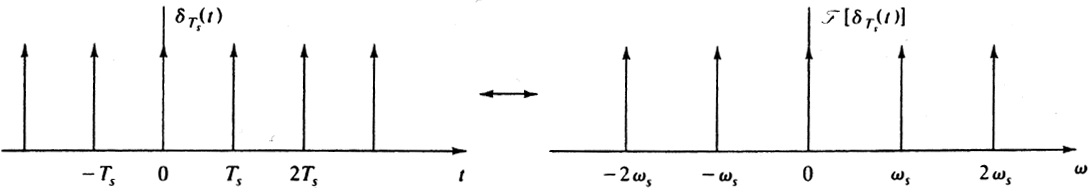
\includegraphics[width=10cm]{../NaT1/bilder/dig_sampler_ideal.png}
	\end{center}

\subsubsection{Abtasttheorem - Nyquist Theorem}
Ein Nachrichtensignal muss mind. mit dem Doppelten seiner Eigenfrequenz abgetastet werden. \\
Ansonsten können sich die Signale im Spektralbereich überlappen.  Um dies zu verhindern wird ein
sogenannter \textbf{Anti-Aliasing Filter} der Abtastung vorgeschaltet.\\
\begin{minipage}[t][2.7cm][c]{8cm}
$ f_s \geq 2 f_M $ \\
$ f_N = 2 \cdot B_M $ \\
$ f_{Nyq} = \frac{f_s}{2}$ \\
$ T_N = \frac{1}{2\cdot B_M} = \frac{1}{f_N} $

\end{minipage}
\begin{minipage}[t][2.7cm][c]{10cm}
	$f_s$ Samplingfrequenz, $[f_s] = Hz$ \\
	$f_M$ Nachrichtenfrequenz, $[f_M] = Hz$ \\
	$B_M$ Nachrichtenbandbreite, $[B_M] = Hz$ \\
	$f_N$ Nyquistrate, $[f_N] = Hz$ \\
	$f_{Nyq}$ Nyquistfrequenz, $[f_{Nyq}] = Hz$ \\
	$T_N$ Nyquistintervall, $[T_N] = s$ \\	
\end{minipage}

Handelt es sich bei dem Nachrichtensignal um ein \textbf{Bandpasssignal}, so kann mit einer noch
kleiner Samplingfrequenz abgetastet werden, dies nennt man \textbf{Subsampling}. \\
Vorgehen: 1. Alle möglichen $n$ bestimmen (ganzzahlig). 2. Alle möglichen Frequenzintervalle für
$f_s$ bestimmen.

\begin{minipage}[t][2cm][c]{10cm}
$$ 1 \leq n \leq \frac{f_u}{f_u - f_l} $$
$$ \frac{2 \cdot f_u}{n} \leq f_s \leq \frac{2 \cdot f_l}{n-1}$$
\end{minipage}
\begin{minipage}[t][2cm][c]{8cm}
	$f_s$ Samplingfrequenz, $[f_s] = Hz$ \\
	$f_l$ Minimale (lower) Nachrichtenfrequenz, $[f_l] = Hz$ \\
	$f_u$ Maximale (upper) Nachrichtenfrequenz, $[f_u] = Hz$ \\
	$n$ Subsampling-Faktor, \textcolor{red}{ganzzahlig} \\
	$n \geq 2$ sonst kein Subsampling möglich
\end{minipage}

Ein weiterer Begriff bezüglich Sampling ist das \textbf{Oversampling}, welches bei \textbf{DAC}s
(Digital-Analog Converter) angewendet wird. \\
Hierbei \textbf{interpoliert} ein DSP zusätzliche Samples, um die Sample-Rate der D/A-Wandlung zu
erhöhen.\\
Folgende Vorteile resultieren daraus: \textbf{Originalgetreueres} Nachrichtensignal, kleinere
\textbf{Filtersteilheit} notwendig.
	\begin{center}
		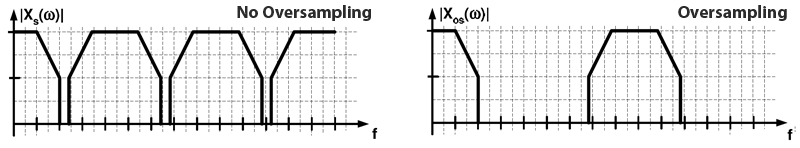
\includegraphics[width=10cm]{../NaT1/bilder/dig_oversampling.png}
	\end{center}

\subsubsection{Natural Sampling\formelbuch{111-5.9}}
Signal mit Periodendauer $T_S$ wird für die Zeit $d$ geschlossen. Amplitude ist bleibt
während Sample nicht konstant. \\
%TODO : Checkliste berechnung des Spektrums für beliebiges Signal

	\begin{center}
		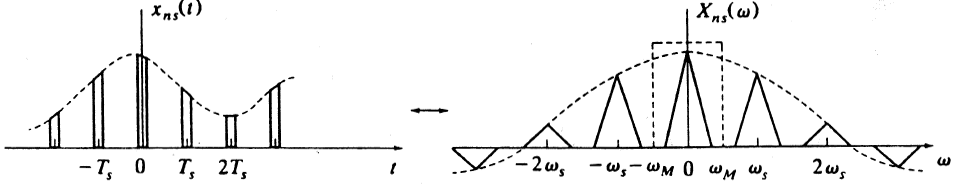
\includegraphics[width=10cm]{../NaT1/bilder/dig_naturalsampling.png}
	\end{center}

\subsubsection{Flat-Top Sampling - Sample \& Hold\formelbuch{112-5.10}}
Das Sample hat die Breite $d$ und bleibt über diese Zeit konstant. \\
Anwendungsbeispiel: A/D-Wandler, Sample \& Hold Schaltung. \\
%TODO : Checkliste berechnung des Spektrums für beliebiges Signal
	\begin{center}
		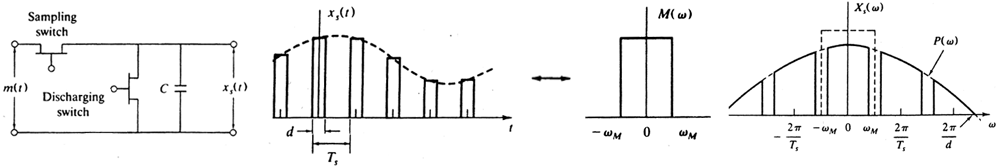
\includegraphics[width=17.5cm]{../NaT1/bilder/dig_flattopsampling.png}
	\end{center}
Das Spektrum des gesampelten Signals wird bei \textbf{höheren Frequenzen} gedämpft, dieses Phänomen
wird als \textbf{Aperture Effect} bezeichnet. Dies kann mit entsprechenden Filtern wieder
korrigiert werden.\\
\hrule
 
\subsection{Quantisierung (Quantizing)\formelbuch{93-5.6}}
	\begin{center}	
		\textbf{Gleichförmig} \hspace{3cm}
		\textbf{Kompressor} \hspace{2.9cm}
		\textbf{$\mu$-Law} \hspace{3cm}
		\textbf{A-Law}  \\
		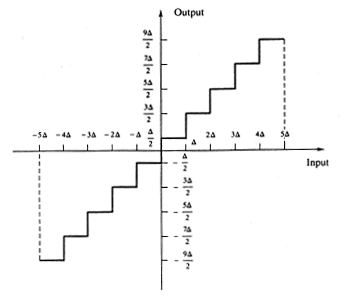
\includegraphics[height=4cm]{../NaT1/bilder/dig_quant_gleichfoermig.png} \hspace{0.5cm}
		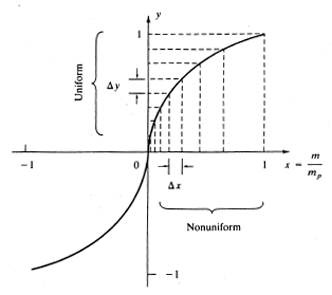
\includegraphics[height=4cm]{../NaT1/bilder/dig_quant_ungleichfoermig.png} \hspace{0.5cm}
		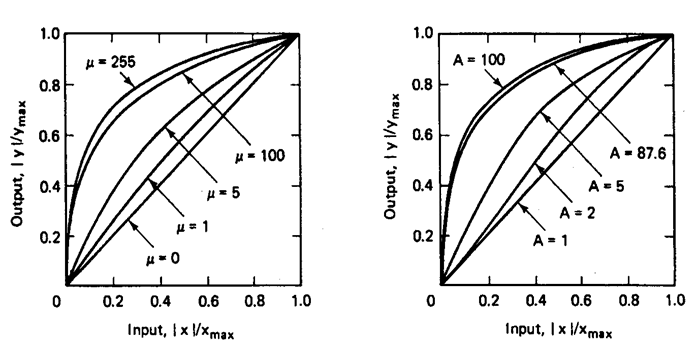
\includegraphics[height=4cm]{../NaT1/bilder/dig_quant_lulaw_ralaw.png}	
	\end{center}
	$\mu$-Law und A-Law sind vor allem bei Signalen mit niedrigem Crest-Faktor von Vorteil: $C = \frac{|x|_{pk}}{x_{RMS}}$

\skriptsubsubsection{Gleichförmige(Uniform) Quantisierung}{93-5.4A}
\begin{minipage}{9cm}
	$$ \Delta = \frac{A_m}{2^{n-1}} = \frac{2 \cdot A_m}{L} \qquad \qquad L = 2^n$$ 
	$$ - \frac{\Delta}{2} \leq q_e \leq \frac{\Delta}{2} \qquad \qquad <q_e^2> = \frac{\Delta^2}{12} =
	\frac{(2 A_m)^2}{L^2 \cdot 12}$$ \vspace{0.1cm}
	$$ \text{SNR} =\frac{S}{N_q}= \frac{S}{q_e^2}$$\\
	$$\text{SNR}_{dB}=10 \log(\text{SNR}) \cdot dB \approx n \cdot 6dB$$
\end{minipage}
\begin{minipage}{9cm}
	$\Delta$ Intervallbreite \\
	$L$ Anzahl Intervalle \\
	$n$ Wortlänge der Samples, [Anzahl Bit] \\
	$A_m$ Amplitude des Nachrichtensignals \\
	$q_e$ Quantisierungsfehler \\
	$<q_e^2>$ Quantisierungsrauschen \\
	SNR Signal-Geräusch Abstand, $[\text{SNR}] = dB$
\end{minipage}

\newpage
\skriptsubsubsection{Ungleichförmige(Nonuniform) Quantisierung}{95-9.5C}
Bei tiefen Nutzsignalen hat die gleichförmige Quantisierung den Nachteil einer schlechten SNR
(Signal - Geräusch Abstand). \\
Beihilfe schafft die Ungleichförmige Quantisierung z.B. bei Telefonie
A-Law-(Europa) oder $\mu$-Law-Codierung (USA, Japan)). \\
Praktisch wird dies mit einem sogenannten \textbf{Kompressor} und einem nachgeschalteten
gleichförmigen Quantisierer realsiert.

\begin{minipage}{9cm}
$$ f_{\mu-Law}(x) = \sgn(x) \frac{\ln(1+\mu\cdot|x|)}{\ln(1+\mu)}$$
$$\text{SNR}_{\mu-Law} \approx 10 \log \dfrac{3 L^2}{[\ln(1 + \mu)]^2}$$
\end{minipage}
\begin{minipage}{9cm}
$$f_{A-Law}(x)=\begin{cases} \frac{A}{1+ \ln A} x & \mbox{wenn }0 \le x \le \frac{1}{A} \\
	\frac{1}{1+ \ln A} + \frac{\ln Ax}{1+ \ln A}, & \mbox{wenn } \frac{1}{A} < x \le 1 \end{cases} $$
$$\text{SNR}_{A-Law} \approx 10 \log \dfrac{3 L^2}{(1+\ln A)^2}$$
\end{minipage}
\hrule

\skriptsubsection{Codierung (Encoding)}{96-5.7}

\skriptsubsubsection{Bandbreitenbedarf von PCM-Signalen}{96-5.8}
\begin{minipage}{9cm}
	$$ f_s > 2 \cdot B_m  \qquad \qquad n = \log_2 L$$ 
	$$ R_B = f_s \cdot n > 2 \cdot n \cdot B_m $$ 
	$$ B_{eff} > B_{PCM} = \frac{1}{2} n \cdot f_s > n \cdot B_m$$
\end{minipage}
\begin{minipage}{9cm}
	$f_s$ Samplingrate, $[f_s] = Hz$ \\
	$n$ Bits pro Sample, \textcolor{red}{ganzzahlig} \\
	$R_B$ Bitrate des PCM-Signals, $[R_B] = \frac{bit}{s}$ \\
	$B_m$ Signalbandbreite, $[B_m] = Hz $ \\
	$B_{PCM}$ Bandbreite PCM Signal, $[B_{PCM}] = Hz $
\end{minipage}


\skriptsubsubsection{Delta Modulation}{97-5.9}
\begin{minipage}{9cm}
$$ \frac{\Delta}{T_s} = \Delta \cdot f_s > \left| \frac{d m(t)}{dt} \right|_{max}$$
$$ (\text{SNR})_0 = 10 \cdot \log\left(\frac{3 f_s^3}{8 \pi^2 f_m^2 f_M}\right) \cdot dB$$ 
$$ <q_e^2> = \frac{\Delta^2}{3} $$ 
\end{minipage}
\begin{minipage}{9cm}
	$f_s$ Samplingrate, $[f_s] = Hz$ \\
	$f_m$ Signalfrequenz, $[f_m] = Hz$ \\
	$f_M$ Grenzfrequenz des TP-Filters, $[f_M] = Hz$ \\
	$B_m$ Signalbandbreite, $[B_m] = Hz $ \\
	$B_{PCM}$ Bandbreite PCM Signal, $[B_{PCM}] = Hz $\\
	$\Delta$ Schritthöhe\\
	$<q_e^2>$ Quantisierungsrauschen \\
	
\end{minipage}

\skriptsubsubsection{Leitungscodierung}{99-5.10}
Je nach Anforderungen (DC-Freie Übertragung, Clock-Rückgewinnung, Störfestigkeit,
Bandbreitenbedarf, Erkennung von Übertragungsfehlern) wird das zu übertragende Signal entsprechend
codiert.

\begin{minipage}{9cm}
	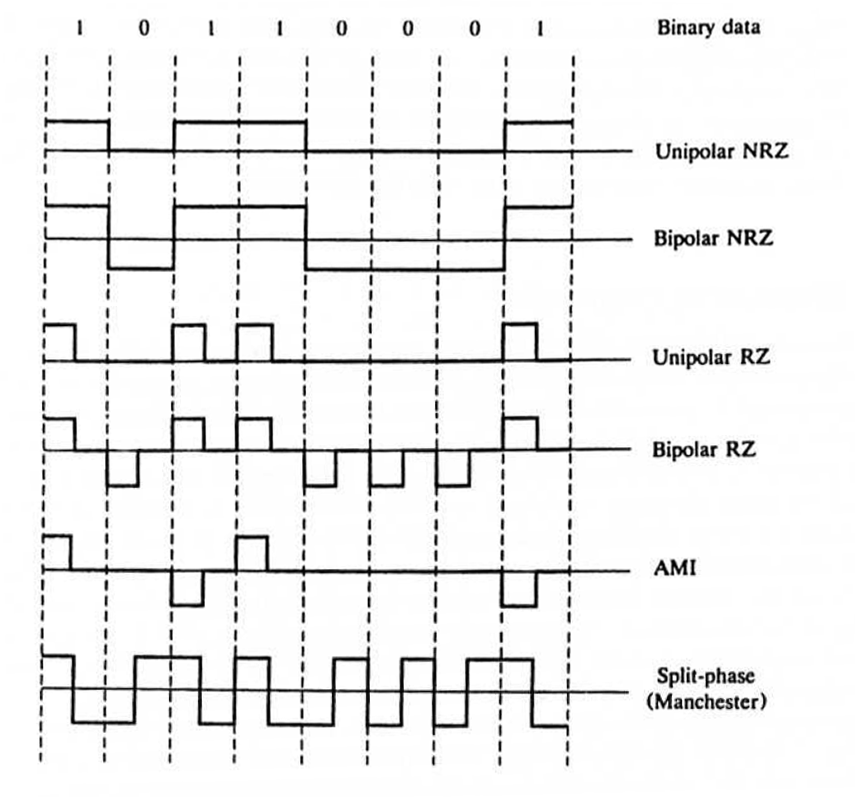
\includegraphics[width=8.7cm]{../NaT1/bilder/dig_leitungscodierung.png}
\end{minipage}
\begin{minipage}{9cm}
	\textbf{Unipolar NRZ(Nonreturn-to-Zero)} \\
	1 = Puls, 0 = kein Puls \\ \\
	\textbf{Bipolar NRZ(Nonreturn-to-Zero)} \\
	1 = positiver Puls, 0 = negativer Puls \\ \\
	\textbf{Unipolar (RZ)Return-to-Zero} \\
	1 = Puls der wieder auf Null zurückspringt, 0 = kein Puls \\ \\
	\textbf{Bipolar RZ} \\
	1 = positiver Puls (kehrt wieder auf Null zurück), 0 = negativer Puls (kehrt wieder auf Null
	zurück)\\ \\
	\textbf{AMI (Alternate Mark Inversion) RZ} \\
	1 = Abwechslungsweise positiver und negatier Puls, 0 = kein Puls. DC-frei\\ \\
	\textbf{Split-Phase (Manchester)} \\
	1 = Positiver Puls mit anschliessend Negativem, 0 = Negativer Puls mit anschliessendem Positivem. DC-frei, einfache Synchronisation
\end{minipage}

\newpage
\skriptsubsubsection{Pulse Shaping und ISI (Intersymbolic Interference)}{101-5.13A}
Da Übertragungskanäle in der Praxis keine idealen Eigenschaften 
(\textbf{limitierte Bandbreite}, Nichtlinearität, Verzerrungen) aufweisen,
werden die - von uns als rechteckig
angenommenen - Pulse verfälscht. Die Pulse werden \textbf{verbreitert} und \textbf{überlappen}
benachbarte Pulse, sodass beim Empfänger eine Unterscheidung der verschiedenen Symbole schwer
fällt. \\
Das oben erwähnte Phänomen wird \textbf{intersymbolic interference} genannt. \\
Abhilfe schafft ein passendes Filter, welches dem Übertragungskanal vorgeschaltet wird. Das Filter
weist eine spezielle Impulsantwort auf, welche bei \textbf{gleichmässigen Zeitabständen}
(Abtastzeiten) Null ist, ausser zum Zeitpunkt Null. Dadurch kann die ISI umgangen werden, wenn dann
genau zu diesen Zeiten abgetastet wird. \\ 

\textbf{Raised-Cosine Filter \formelbuch{103}} \\
Dieses Filter schafft Abhilfe bei ISI. Obwohl dies auch mit einem Idealen Filter
(Sinc-Frequenzgang) möglich wäre, wird ein Raised-Cosine mit folgenden Vorteilen eingesetzt:
\begin{itemize}
  \item Raised-Cosine-Puls fällt schneller ab als Sinc-Puls
  \item Raised-Cosine ist zwar auch akausal, aber in der Praxis einfacher realisierbar 
\end{itemize}

\begin{minipage}{9cm}
$$ f_B = \frac{1 + \alpha}{2 T} Hz \qquad \qquad \frac{1}{T} = \frac{2 f_B}{1 + \alpha}$$
\end{minipage}
\begin{minipage}{9cm}
	$f_B$ benötigte Bandbreite, $[f_B] = Hz$ \\
	$\frac{1}{T}$ Pulsrate, $[\frac{1}{T}] = $ "Pulse pro Sekunde" \\
	$\alpha$ roll-off-Faktor, $[\alpha] = 1$ 
\end{minipage}

\begin{center}  
		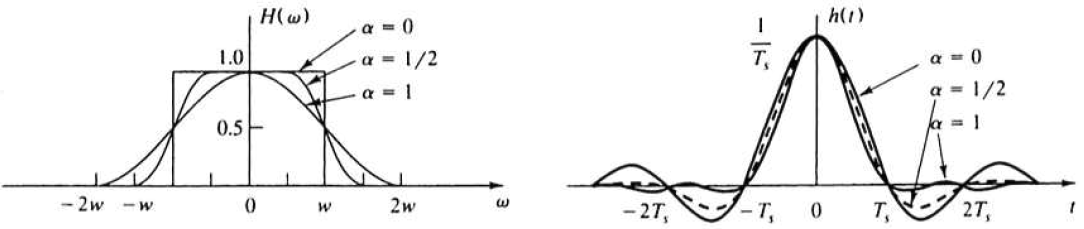
\includegraphics[height=3.2cm]{../NaT1/bilder/dig_raisedcosinefilter.png}
\end{center}


$$ 
h(t) = \frac{1}{T_s} = \left( \frac{\sin{W t}}{W t} \right) \left[ \frac{\cos{\alpha W t}}{1
- (2 \alpha W t / \pi)^2}\right]
\quad \laplace \quad
H(\omega) = \begin{cases}
	1 			
		&  	0 \leq | \omega | \leq (1-\alpha) W       \\
	\frac{1}{2} \left( 1 - \sin\left[ \frac{\pi}{2 \alpha W} (| \omega | - W)\right] \right)      
		&	(1-\alpha) W \leq | \omega | \leq (1+\alpha) W       \\
	0
		& 	| \omega | > (1+\alpha) W
            \end{cases}
$$


% 
% Vorteil Raised-Cosine zu Sinc: RCosine fällt schneller ab (wenn t gegen unendlich). \\
% RCosine ist zwar auch akausal aber kann viel besser approximiert(praktisch realisiert) werden als
% ein sinc, da er schneller abfällt!

\skriptsubsubsection{Digitale Trägermodulation}{104-5.14}
\begin{minipage}{9cm}
	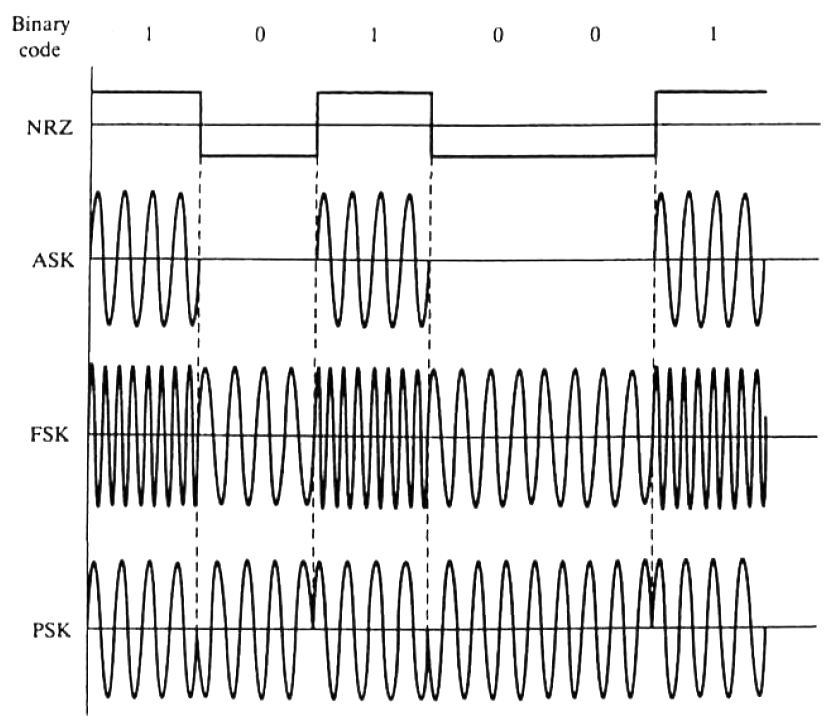
\includegraphics[width=8.7cm]{../NaT1/bilder/dig_traegermodulation.png}
\end{minipage}
\begin{minipage}{9cm}
	Weil Binäre Nachrichtensignale selbst zu kleine Frequenzen aufweisen, sind sie nicht geeignet um
	z.B. über den Äther zu schicken. Abhilfe schafft die binäre Trägermodulation. 
	\vspace{1cm}  \\
	\textbf{ASK - Amplitude-Shift Keying} \\
	$$x_c(t) = \begin{cases}
           A \cos(\omega_c t) & \textbf{symbol 1} \\
           0 & \textbf{symbol 0}
           \end{cases} $$ \\
	\textbf{FSK - Frequency-Shift Keying} \\
	$$x_c(t) = \begin{cases}
           A \cos(\omega_{c1} t) & \textbf{symbol 1}     \\         
           A \cos(\omega_{c2} t) & \textbf{symbol 0}
           \end{cases} $$ \\
	\textbf{PSK - Phase-Shift Keying} \\
	$$x_c(t) = \begin{cases}
           A \cos(\omega_{c} t) & \textbf{symbol 1}        \\      
           A \cos(\omega_{c} t + \pi) & \textbf{symbol 0}
           \end{cases} $$ \\
\end{minipage}



\newpage
\section{Übungsverzeichnis}

\subsection{Einführung}
	\begin{tabular}{|p{9cm}|p{2.5cm}|p{3.5cm}|p{2cm}|}
	\hline
	\textbf{Thema} & \textbf{Hausübung} & \textbf{Schaum} & \textbf{Praktikum} \\ \hline
	Dezibel & 2.1 &  &  \\ \hline
	Fouriertransformierte & 2.5, 2.6, 3.1, 3.2  & 1.10, 1.14, 1.15, 1.28 &  \\
	\hline Komplexe Fourierreihe & 2.3, 2.4 & & \\ \hline
	Modulationssatz & 2.7 & & \\ \hline
	Crest-Faktor & 1.1 & & \\ \hline
	\end{tabular}

\subsection{LTI-Systeme}
	\begin{tabular}{|p{9cm}|p{2.5cm}|p{3.5cm}|p{2cm}|}
	\hline
	\textbf{Thema} & \textbf{Hausübung} & \textbf{Schaum} & \textbf{Praktikum} \\ \hline
	LTI: Linearität und Zeitinvarianz & 3.3, 3.4 & 2.1, 2.2 &  \\ \hline
	LTI: RL-Filter & 3.5 & 2.11 &  \\ \hline
	\end{tabular}

\subsection{Amplitudenmodulation}
	\begin{tabular}{|p{9cm}|p{2.5cm}|p{3.5cm}|p{2cm}|}
	\hline
	\textbf{Thema} & \textbf{Hausübung} & \textbf{Schaum} & \textbf{Praktikum} \\ \hline
	DSB-SC &  &  & 3-6.2 \\ \hline
	OAM: Koharände Demodulation & & 3.5 & 4 \\ \hline
	OAM: Spitzenwertdetektor & 5.2 & 3.6 & 4 \\ \hline
	Ordinary AM & 5.1 & 3.4 & 3 \\ \hline
	QAM & 6.3  & 3.15 & 4 \\ \hline
	SSB-AM: Demodulation mit koharäntem Demodulator & 5.1, 6.2 & 3.9 & 4 \\
	\hline SSB-AM: Modulation mit Eintonsignal & 6,1 & 3.7, 3.8 & 4-7.2 \\ \hline
	\end{tabular}

\subsection{Winkelmodulation - FM/PM}
	\begin{tabular}{|p{9cm}|p{2.5cm}|p{3.5cm}|p{2cm}|}
	\hline
	\textbf{Thema} & \textbf{Hausübung} & \textbf{Schaum} & \textbf{Praktikum} \\ \hline
	FM/PM: Bandbreite & 7.5, 7.6 & 4.9, 4.10 & 5-7.3 \\ \hline
	FM/PM: Bandbreitenänderung & 7.8 & 4.13 & 5-7.3 \\ \hline
	FM/PM: Frequenz- \& Phasenabweichung & 7.2 & 4.2 & 5-7.1 \\ \hline
	FM/PM: Leistung des modulierten Signals & 7.4 & 4.6 &  \\ \hline
	FM/PM: Modulationsindex & 7.6, 7.7 & 4.10, 4.11, 4.12 &  \\ \hline
	FM/PM: Momentanfrequenz & 7.1 & 4.1 & 5-7.1 \\ \hline
	PM: Nichtlinearität & 7.3 & 4.4 &  \\ \hline
	\end{tabular}

\subsection{Digitale Übermittlung analoger Signale}
	\begin{tabular}{|p{9cm}|p{2.5cm}|p{3.5cm}|p{2cm}|}
	\hline
	\textbf{Thema} & \textbf{Hausübung} & \textbf{Schaum} & \textbf{Praktikum} \\ \hline
	Delta-Modulation & 11 & 5.21, 5.22, 5.23, 5.24 & 7 \\ \hline
	ISI, Pulse-Shaping (Raised Cosine) &  & 5.36 &  \\ \hline
	PCM: Quantisierungsrauschen, SNR & 10.6 & 5.15, 5.16 &  \\ \hline
	PCM: Samplerate, Quantisierung, Bitrate & 10.3 & 5.12 &  \\ \hline
	PCM: Samplerate, Wortbreite, Bitdauer & 10.5 & 5.14 &  \\ \hline
	PCM: SNR und Bitrate einer CD & 10.8 & 5.17 &  \\ \hline
	PCM: Wortbreite & 10.4, 10.7 & 5.13, 5.16 &  \\ \hline
	Quantisierung: Ungleichförmig: A-Law, $\mu$-Law; SNR & 10.9, 10.10 & 5.18, 5.19
	& 6 \\ \hline Sampling: Basisbandsignale & 9.4a & 5.8 &  \\ \hline
	Sampling: Flat-top Sampling & 10.2 & 5.1 & 6 \\ \hline
	Sampling: Natural Sampling & 10.1 & 5.9 & 6 \\ \hline
	Sampling: Nyquist-Frequenz/-Rate/-Intervall & 9.1, 9.2 & 5.6 &  \\ \hline
	Sampling: Subsampling & 9.3, 9.4b & 5.7, 5.8 &  \\ \hline
	Sampling: Unterabtastung & & 5.3 &  \\ \hline
	Leistungscodierung & 12.1 && \\ \hline
	\end{tabular}


\subsection{Multiplexverfahren}
	\begin{tabular}{|p{9cm}|p{2.5cm}|p{3.5cm}|p{2cm}|}
	\hline
	\textbf{Thema} & \textbf{Hausübung} & \textbf{Schaum} & \textbf{Praktikum} \\ \hline
	Multiplexing: Zeitmultiplex (TDM) & 13 & 5.31 &  \\ \hline
	\end{tabular}



\end{document}
